\documentclass[11pt]{beamer}
\usepackage[ngerman]{babel}
\usepackage[utf8]{inputenc}
\usepackage[T1]{fontenc}
\usepackage{lmodern}
\usepackage{multicol}
\usepackage{csquotes}
\usetheme{Singapore}
\begin{document}
	\author{Andreas Windorfer}
	\title{Tango Bäume}
	%\subtitle{}
	%\logo{}
	%\institute{}
	\date{\today}
	%\subject{}
	%\setbeamercovered{transparent}
	%\setbeamertemplate{navigation symbols}{}
	\begin{frame}{}
		\titlepage
	\end{frame}
		\begin{frame} {Übersicht}
		\tableofcontents[]   
		
	\end{frame}
	
	\section{Binärer Suchbaum}
	
	
		\begin{frame} {Binärer Suchbaum}
			\begin{figure}[h]
				\centering
				\includegraphics[width=0.75\textwidth]{"Medien/pres/ioSuchbaum"}
			\end{figure}    
		\end{frame}

			\begin{frame} {Binärer Suchbaum}
			\begin{figure}[h]
				\centering
				\includegraphics[width=0.75\textwidth]{"Medien/pres/suchbaum2_2"}
			\end{figure}    
		\end{frame}

			\begin{frame} {Binärer Suchbaum}
			\begin{figure}[h]
				\centering
				\includegraphics[width=0.75\textwidth]{"Medien/pres/VorgängerNachfolger"}
			\end{figure}    
		\end{frame}
	
	\begin{frame} {Binärer Suchbaum}
			\begin{figure}[h]
				\centering
				\includegraphics[width=0.75\textwidth]{"Medien/pres/LinksRechtsRotation"}
			\end{figure}    
		\end{frame}	
	
	\section{Dynamische Optimalität}
	
		\begin{frame} {Übersicht}
			\tableofcontents[currentsection]   
		\end{frame}
	
	   
    
    
  \begin{frame} {	\textit{access}$\left(k\right)$ Operation}
    \begin{block}{Parameter / Rückgabe}
    	\begin{itemize}
    		\item Parameter $k$: Schlüssel im BST (Schlüsselmenge $K$)
    		\item Rückgabe: Knoten mit Schlüssel $k$
      \end{itemize}
    			
    \end{block}	
  \end{frame}	
     
     \begin{frame} {	\textit{access}$\left(k\right)$ Operation}
     	\begin{block}{Einschränkungen}
     		Ein Zeiger $p$ (berührter Knoten) in die Struktur:
     		\begin{itemize}
     			\item Setze $p$ auf ein Kind von $p$ 
     			\item Setze $p$ auf den Elternknoten von $p$ 
     			\item Rotationen 
     		\end{itemize}	
     	\end{block}	
     	\pause 
     	\begin{block}{Berechnung der Kosten}
     		
     		Einheitskosten von \enquote{1}.
     	\end{block}	    	
     \end{frame}	    
     
      
  \begin{frame} {	Zugriffsfolgen} 
    \begin{block}{Zugriffsfolgen}
    	\begin{itemize}
    		\item   $X = x_1, x_2,..., x_m$ , mit $\forall i \in \{1,2,..,m\}: x_i \in K$
    		\item  \textit{access}$\left(x_1\right)$,   \textit{access}$\left(x_2\right)$, ....,  
    		\textit{access}$\left(x_m\right)$  
    	\end{itemize}
    \end{block}			
	\pause
   \begin{block}{dynamische BST}
	 \begin{itemize}
		\item Anpassung der Struktur 	 
 	\end{itemize}
   \end{block}			
 \begin{block}{Kostenrechnung}
		\textit{Anzahl der Einzelschritte} + $m$	 
\end{block}		
\end{frame}	  
  \begin{frame} {	dynamisch Optimal} 
	\begin{block}{$\mathit{OPT}\left(X\right)$}
		Niedrigste Kosten zum Ausführen von $X$ 
	\end{block}			
	\pause
	\begin{block}{dynamisch Optimal}
	BST mit Kosten von  $O\left(\mathit{OPT}\left(X\right)\right)$, für beliebige $X$
	\end{block}			
	\begin{block}{c-competitive}
		BST mit Kosten von  $O\left(c \cdot \mathit{OPT}\left(X\right)\right)$, für beliebige $X$	 
	\end{block}		
\end{frame}	  
    
\section{Tango Baum}

 \begin{frame} {Tango Baum} 
 	\begin{block}{Eigenschaten}
 		\begin{itemize}
 			\item 	Aus BSTs bestehender BST
 			\item $\log\left(\log\left(n\right)\right)$-competitive		
 		\end{itemize}
    \end{block}
	\begin{block}{Literatur}
	Erik D. Demaine, Dion. Harmon, John. Iacono, and Mihai. Patrascu.
	Dynamic optimality-almost. SIAM Journal on Computing, 37(1):240
	251, 2007.
    \end{block}
\end{frame}	  
 \begin{frame} {Interleave Lower Bound} 
 	\begin{block}{Motivation}
 	\begin{itemize}
 		\item Berechnung einer unteren Schranke zu $\mathit{OPT\left(X\right)}$
 		\item Beweis der $\log\left( \log \left(n\right)\right)$-competitiveness	
 	\end{itemize}
     \end{block}
\end{frame}	  

 \begin{frame} {Lower Bound Tree} 
	\begin{block}{Definition}
		  Zu $X = x_1,x_2,.,x_m$ und $K = \{k \in \mathbb{N} \vert k \textit{ ist in $X$ enthalten}\}$\\
		  \pause
		  ist der komplette BST $P$ mit der Schlüsselmenge $K$ der LBT. 
		 
	\end{block}
\end{frame}

\begin{frame} {Beispiel LBT} 
\begin{figure}[H]
	\centering
	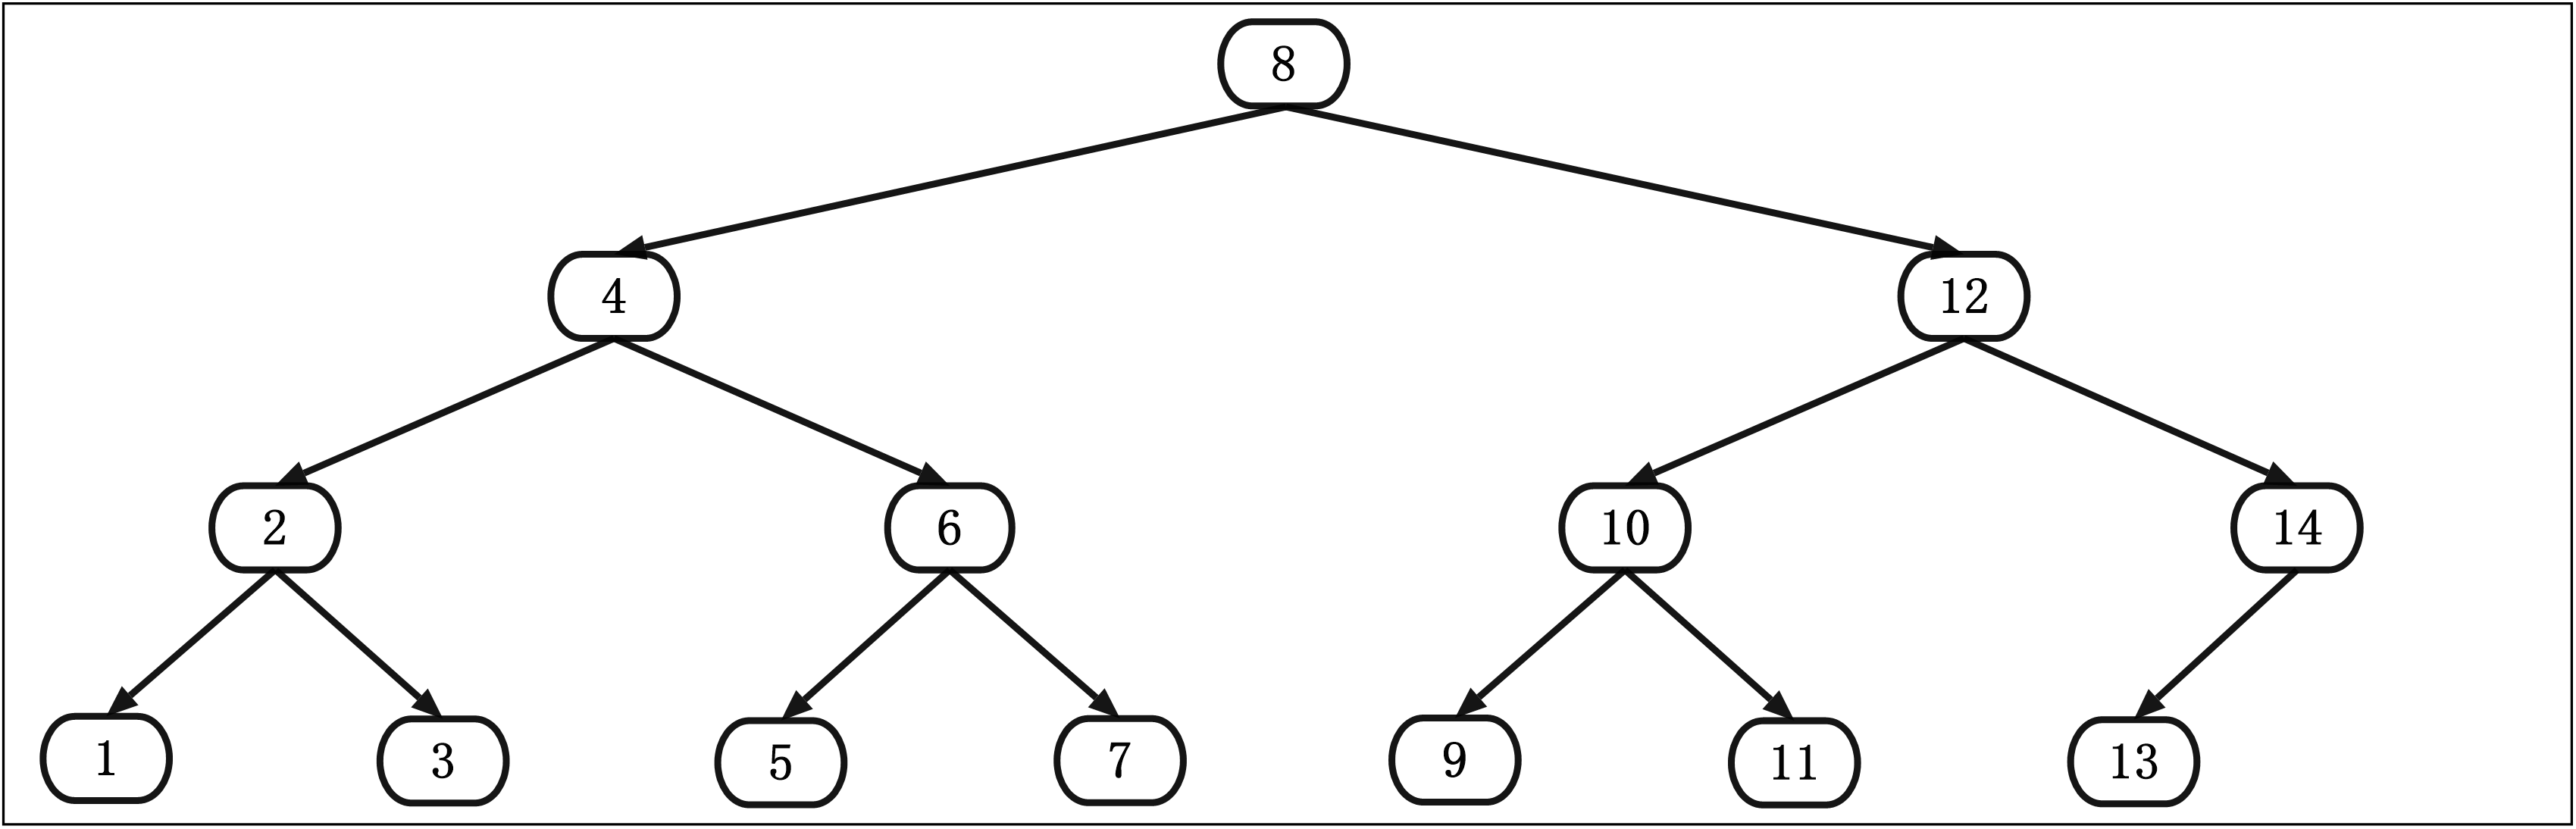
\includegraphics[width=1\textwidth]{Medien/pres/lowerBoundTree}
	\caption{Der Lower Bound Tree zur Zugriffsfolge $1 ,2, .., 14$.  }
	\label{fig:demlowerBoundTree}
\end{figure}
\end{frame}		


 \begin{frame} {Lower Bound Tree} 
	\begin{block}{Linke Region eines Kontens $v$}
	      Schlüssel des linken Teilbaumes von $v$ und \textit{key}$\left(v\right)$	
	\end{block}
    \begin{block}{Linke Region eines Kontens $v$}
	Schlüssel des rechten Teilbaumes von $v$
	\end{block}
	\begin{block}{Interleave durch $v$}
		$x_{i-1}$ liegt in der linken Region und $x_i$ in der rechten,\\
		oder umgekehrt.
    \end{block}
\end{frame}

 \begin{frame} {Lower Bound Tree} 
	\begin{block}{\textit{inScore} $\left(X, v\right)$}
		Anzahl der Interleaves durch $v$
	\end{block}
	\begin{block}{$\mathit{IB}\left(X\right)$}
		$\mathit{IB}\left(X\right) = \sum_{u \in U} \mathit{inScore}\left(X, u\right)$
	\end{block}
\end{frame}

\begin{frame} {Transition Points} 
	$T_0$ Startzustand, $T_i$ nach ausführen von \textit{access} $x_i$.
	\pause
	$j \in {0,1,..m}$\\
	\bigskip
	Zu jedem Knoten $u$ aus $P$, mit nicht leerer rechter Region,\\
	existiert ein transition point in $T_j$ 
	
	
\end{frame}

\begin{frame} {Transition Points} 
	Sei $v$ der Transition Point zu $u$ und $T_j$
	\begin{enumerate}
		\item Im Pfad von der Wurzel zu $v$ ist ein Knoten mit einem Schlüssel aus der linken Region von $u$ enthalten.
		\item Im Pfad von der Wurzel zu $v$ ist ein Knoten mit einem Schlüssel aus der rechten Region von $u$ enthalten.
		\item Kein anderer Knoten mit kleinerer Tiefe erfüllt die Eigenschaften eins und zwei. 
	\end{enumerate}	
\end{frame}
\begin{frame} {Transition Points} 
	Sei $U$ die Menge der Knoten in $P$ mit einer nicht leeren rechten Region.
	\begin{itemize}
		\item Lemma 1: Es gibt zu jedem Knoten $u \in U$ genau einen transition point in $T_j$. 	
		\item Lemma 2: Wird ein transition point nicht berührt, so ist er noch immer der transition point des selben Knotens.
		\item Lemma 3: Ein Knoten kann nicht der transition point mehrerer Knoten sein. 
	\end{itemize}	
\end{frame}

\begin{frame} {Beweis Lemma 1}
\begin{enumerate}
	\item  $l$	ist der kleinste Schlüssel der linken Region
	\item  $r$	ist der größte Schlüssel der rechten Region
	\pause
	\item der Teilbaum mit der Wurzel $u$ enthält genau die Schlüssel aus $K^r_l = \{k \in K \vert k \in \left[l,r\right]\}$
	\pause
	\item  $v_l$ ist der Vorfahre der Schlüssel der linken Region
	\item  $v_r$ ist der Vorfahre der Schlüssel der rechten Region
	\item  $w$ ist der gemeinsame Vorfahre dieser Schlüssel
\end{enumerate}	
\end{frame}

\begin{frame} {Beweis Lemma 1}
\begin{figure}[H]
	\centering
	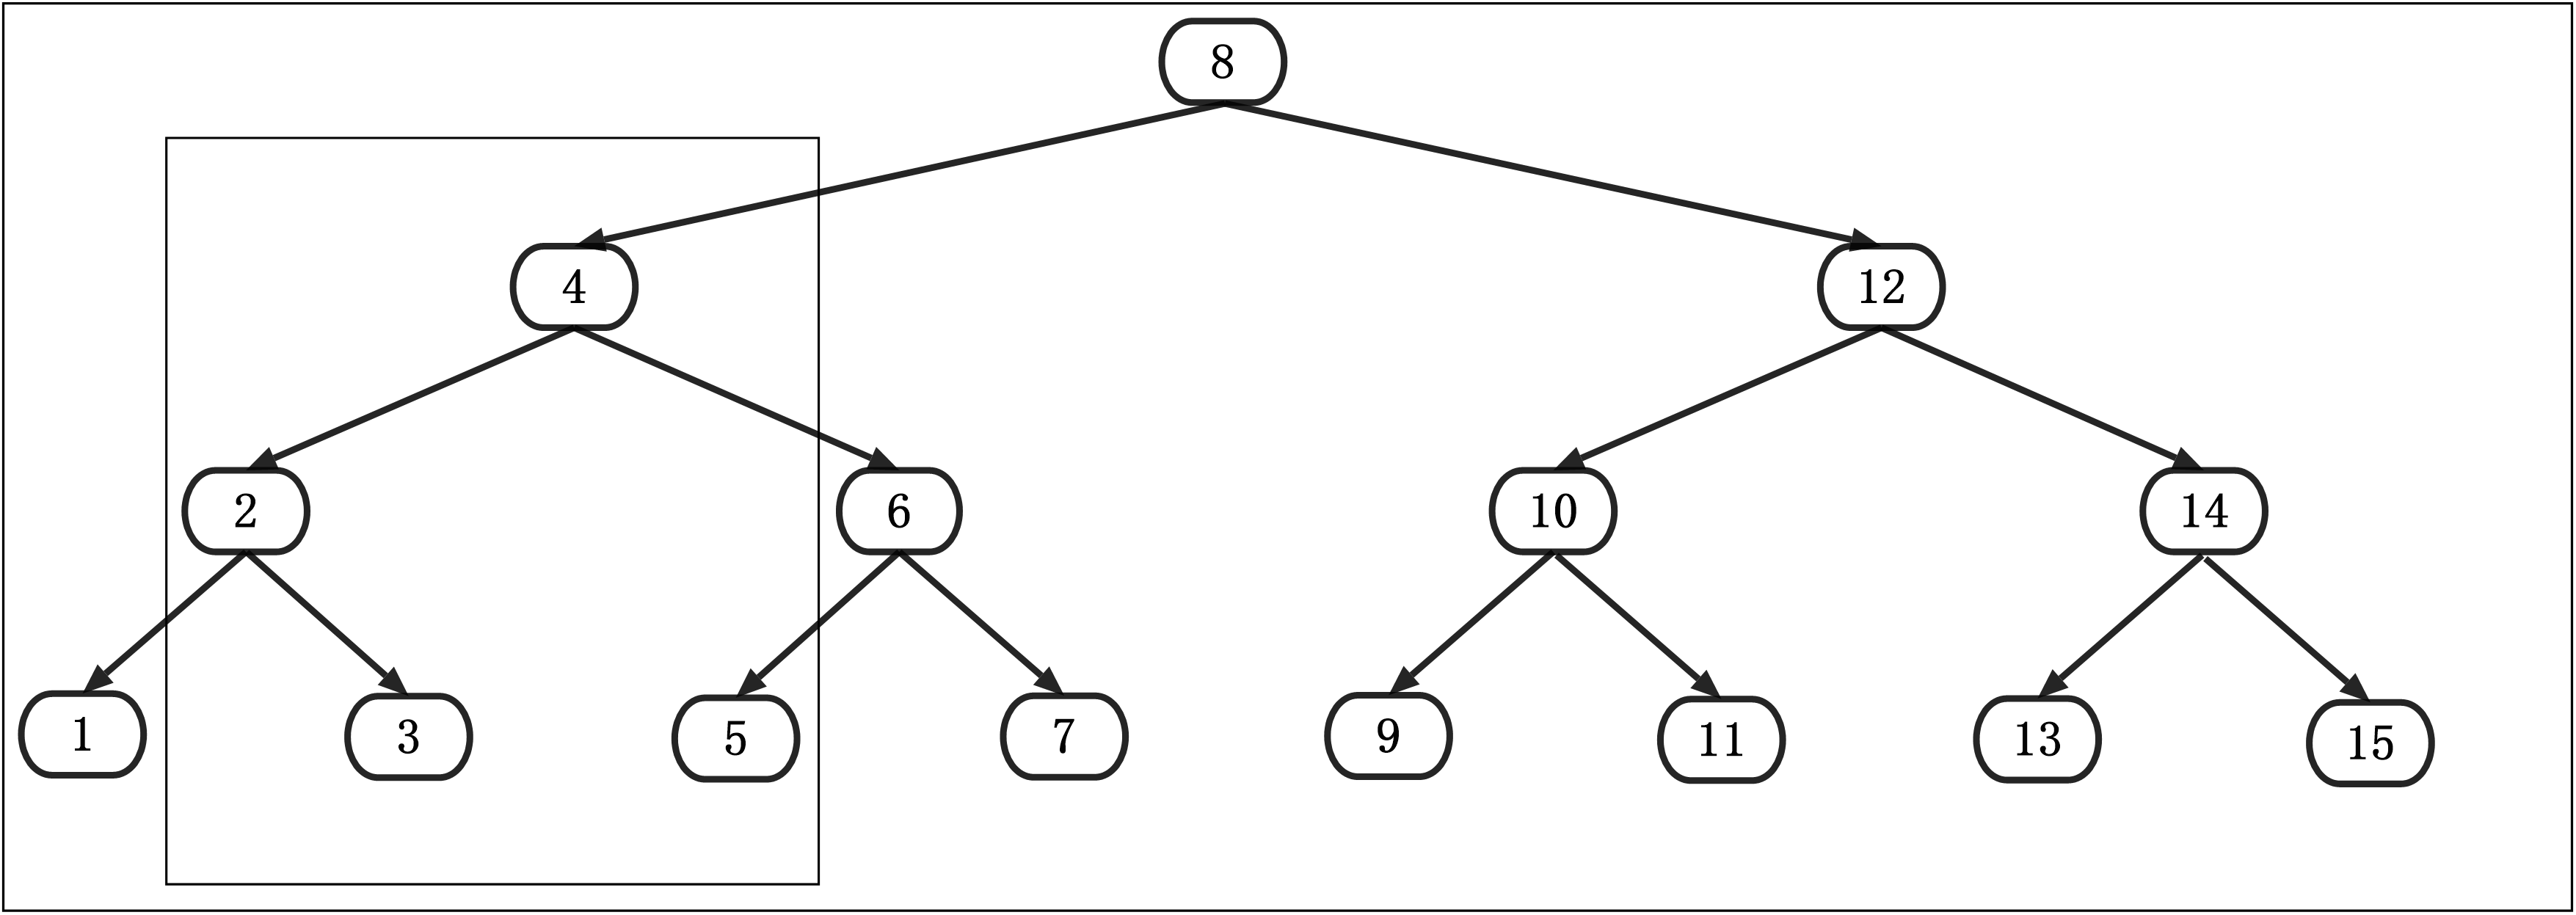
\includegraphics[width=1\textwidth]{Medien/pres/linksRechts1}
\end{figure}
\end{frame}
\begin{frame} {Beweis Lemma 1}
	\begin{figure}[H]
		\centering
		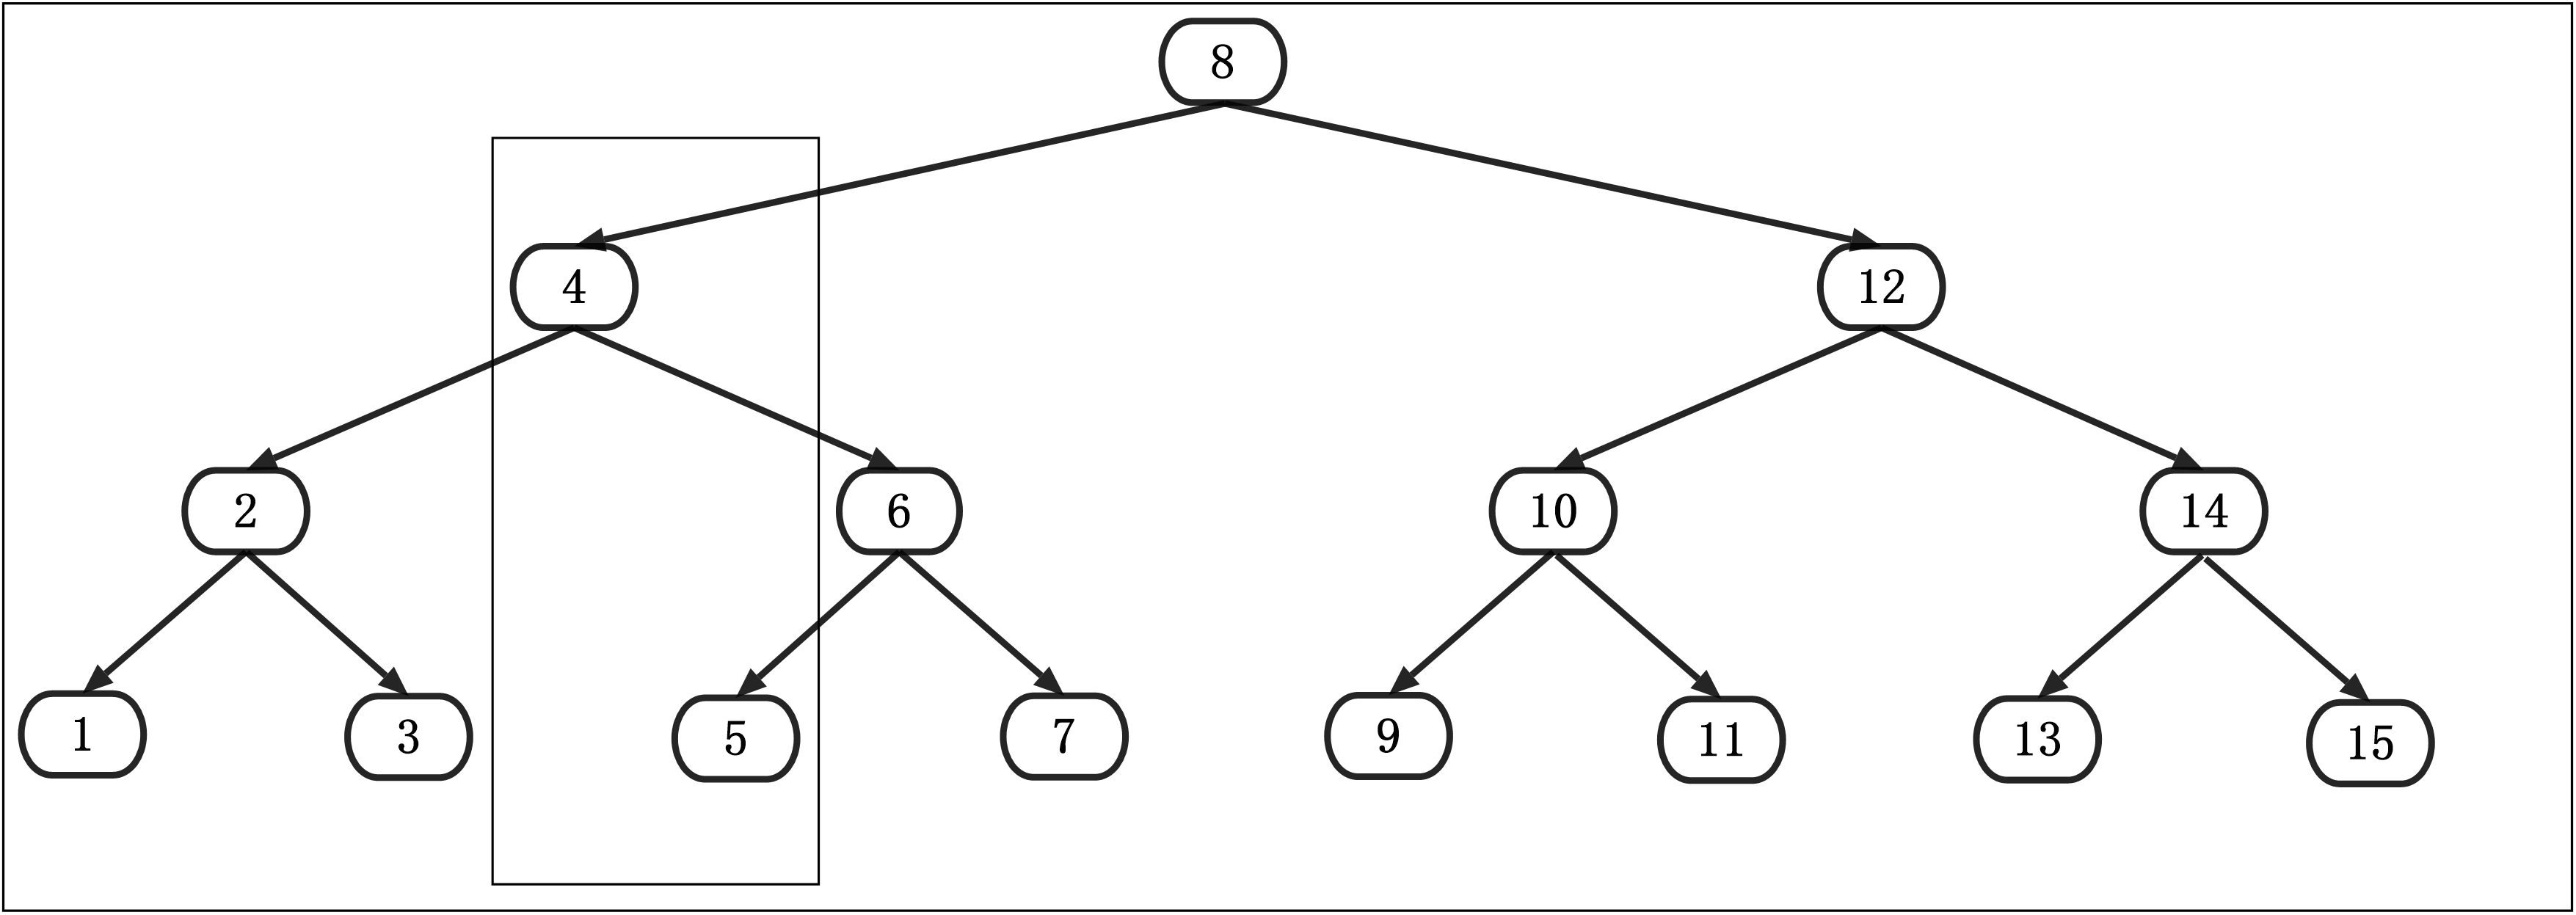
\includegraphics[width=1\textwidth]{Medien/pres/linksRechts2}
	\end{figure}
\end{frame}

\begin{frame} {Beweis Lemma 1}
	\begin{enumerate}
			\item  $l$	ist der kleinste Schlüssel der linken Region
		\item  $r$	ist der größte Schlüssel der rechten Region
		\pause
		\item der Teilbaum mit der Wurzel $u$ enthält genau die Schlüssel aus $K^r_l = \{k \in K \vert k \in \left[l,r\right]\}$
		\pause
		\item  $v_l$ ist der Vorfahre der Schlüssel der linken Region
		\item  $v_r$ ist der Vorfahre der Schlüssel der rechten Region
		\item  $w$ ist der gemeinsame Vorfahre dieser Schlüssel
		\item  $w = v_l$ bzw. $w = v_r$	
		\item  Transition point ist $v_r$ bzw. $v_l$ 
	\end{enumerate}	
\end{frame}
\begin{frame} {Transition Point Zuordnung}
	\begin{figure}[H]
		\centering
		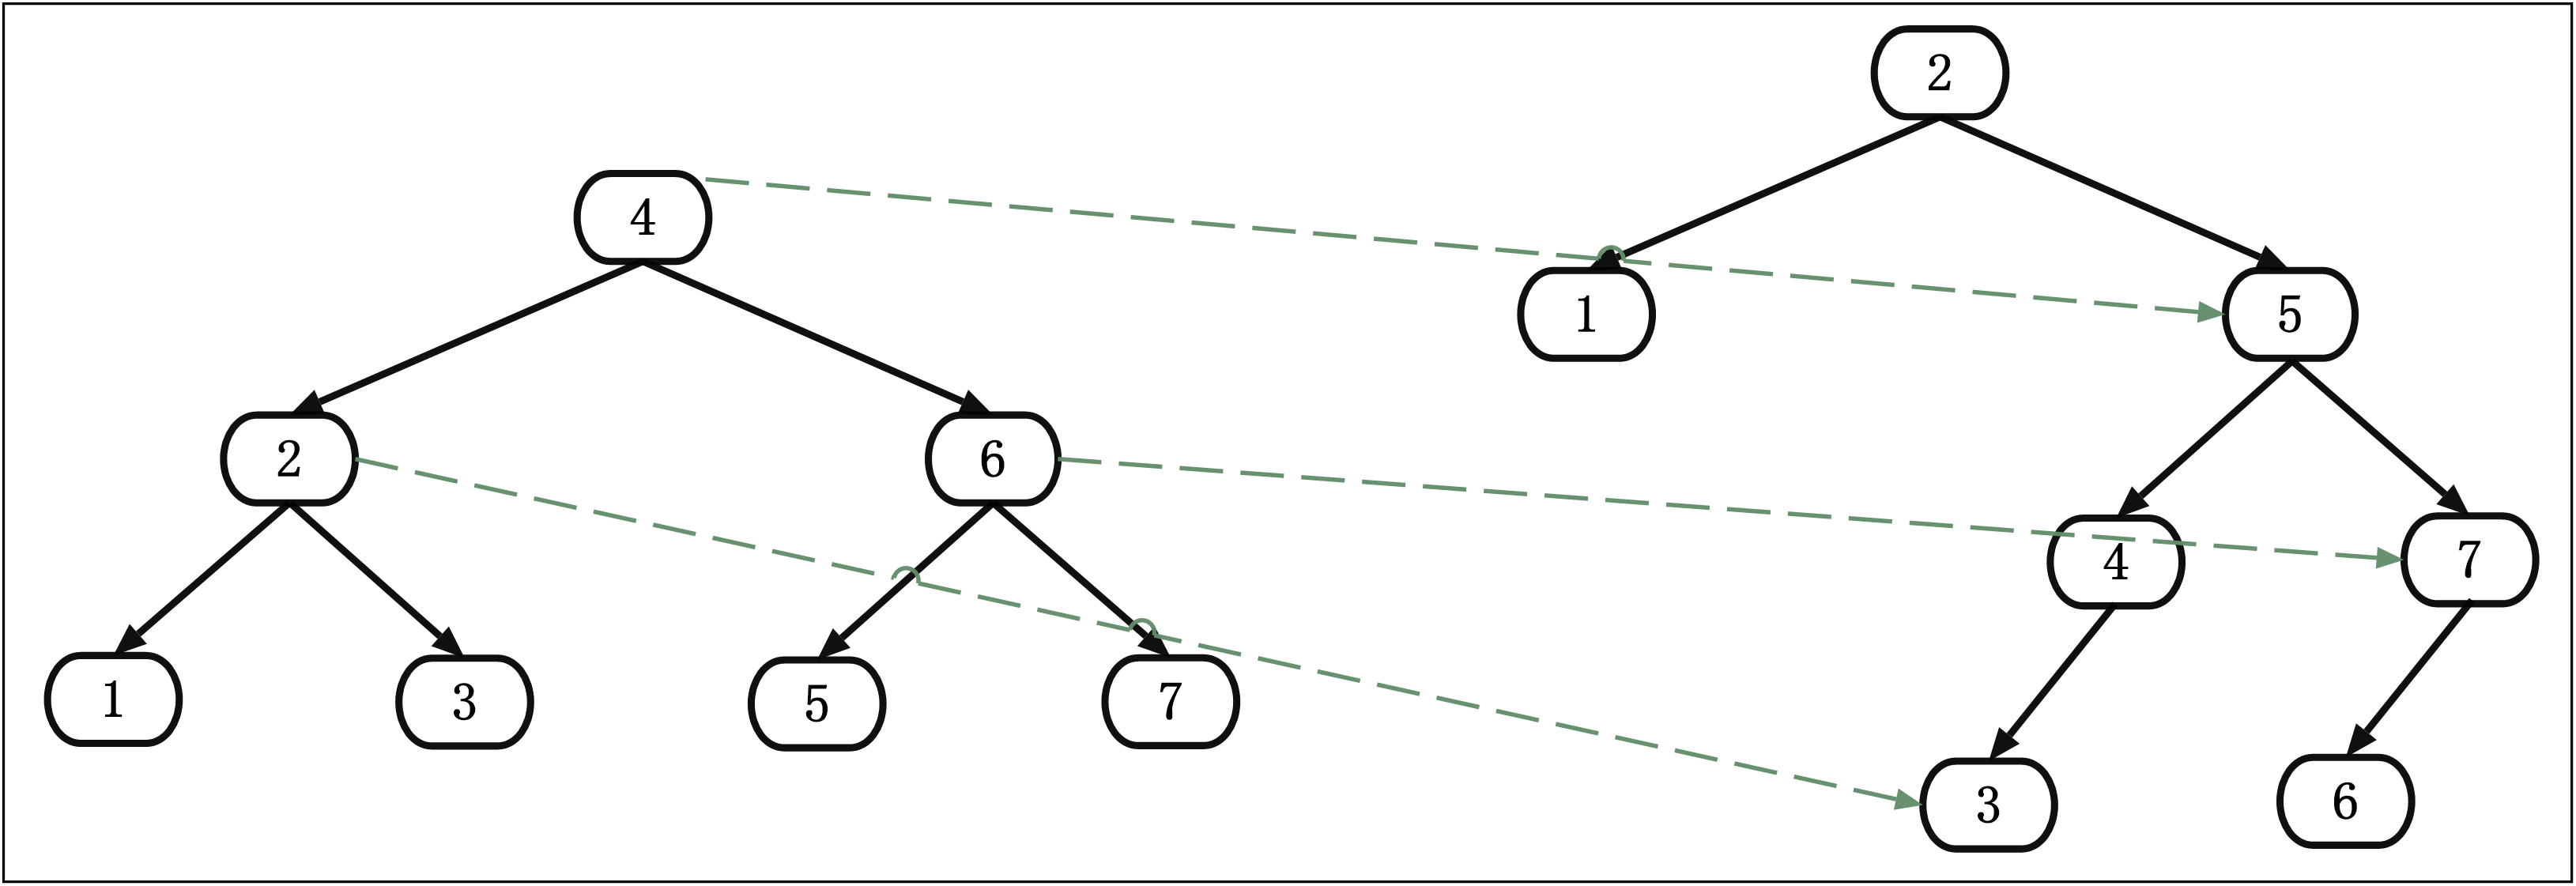
\includegraphics[width=1\textwidth]{Medien/pres/transitionPoints}
		\caption{Links ein Lower Bound Tree, rechts ein BST }
	\end{figure}
\end{frame}

\begin{frame} {Satz Interleave Lower Bound}
		Sei $X = x_0, x_1,.., x_m$  eine Zugriffsfolge und $n$ die Anzahl der Knoten im zu $X$ erstellten Lower Bound Tree Y. Dann gilt\\	
	$\mathit{OPT}\left(X\right) \geq \mathit{IB}\left(X\right) /2 - n$ .
	
\end{frame}

\begin{frame} {Beweis Interleave Lower Bound}
	\begin{enumerate}
		\item Zählen der Berührungen von Transition Points
		\item Die Anzahl der Berührungen kann für jeden Knoten einzeln bestimmt werden. (Lemma $5.1$ und $5.3$)
		\pause
		\item Betrachteter Knoten $u$. \mbox{$X{^r_l}' = x_{i_0},x_{i_1},..,x_{i_p}$} bilden
		\item $\mathit{inScore}\left(X, u\right) = p$
		\pause
		\item  Sei $q \in \mathbb{N}$ mit $1 \leq q \leq \lfloor p / 2 \rfloor$
		\pause
		\item  Es folgen mindestens $\lfloor p/2 \rfloor \geq p/2 - 1$ Berührungen des transition points von $u$
		\pause
		\item $\mathit{IB}\left(X\right) /2 - \vert U \vert \geq \mathit{IB}\left(X\right) /2 - n$
	\end{enumerate}
	
\end{frame}

\end{document}